%-----------------------------------------------------------------------------
%
%               Template for sigplanconf LaTeX Class
%
% Name:         sigplanconf-template.tex
%
% Purpose:      A template for sigplanconf.cls, which is a LaTeX 2e class
%               file for SIGPLAN conference proceedings.
%
% Guide:        Refer to "Author's Guide to the ACM SIGPLAN Class,"
%               sigplanconf-guide.pdf
%
% Author:       Paul C. Anagnostopoulos
%               Windfall Software
%               978 371-2316
%               paul@windfall.com
%
% Created:      15 February 2005
%
%-----------------------------------------------------------------------------


\documentclass{sigplanconf}

% The following \documentclass options may be useful:

% preprint      % Remove this option only once the paper is in final form.
% 10pt          To set in 10-point type instead of 9-point.
% 11pt          To set in 11-point type instead of 9-point.
% authoryear    To obtain author/year citation style instead of numeric.

\usepackage{amsmath}
\usepackage{natbib}
\usepackage{graphicx}
\usepackage{wrapfig}
\usepackage{caption}
\usepackage{url}


\begin{document}

\special{papersize=8.5in,11in}
\setlength{\pdfpageheight}{\paperheight}
\setlength{\pdfpagewidth}{\paperwidth}

\conferenceinfo{CONF 'yy}{Month d--d, 20yy, City, ST, Country} 
\copyrightyear{20yy} 
\copyrightdata{978-1-nnnn-nnnn-n/yy/mm} 
\doi{nnnnnnn.nnnnnnn}

% Uncomment one of the following two, if you are not going for the 
% traditional copyright transfer agreement.

%\exclusivelicense                % ACM gets exclusive license to publish, 
                                  % you retain copyright

\permissiontopublish             % ACM gets nonexclusive license to publish
                                  % (paid open-access papers, 
                                  % short abstracts)

\titlebanner{banner above paper title}        % These are ignored unless
\preprintfooter{short description of paper}   % 'preprint' option specified.

\newcommand{\pname}{KinEdit}

\title{\pname{}: A Tool to Help Developers Refactor Manually}
% \subtitle{View and edit all contexts referring to a common identifier}

\authorinfo{Josh Terrell}
           {California Polytechnic University, San Luis Obispo}
           {jmterrel@calpoly.edu}
% \authorinfo{Name2\and Name3}
%            {Affiliation2/3}
%            {Email2/3}

\maketitle

\begin{abstract}
Some developers do not trust automated refactoring tools to refactor correctly.
Refactoring without tools can be a cumbersome and error-prone process.
It is possible for a tool to support developers in refactoring without
requiring them to trust in automated code manipulation.
This paper contributes \pname{}---a tool which is designed to help developers
manually refactor more quickly, with higher quality,
and without requiring the developers' trust.
% problem. why propblem is problem. startling sentence (make claim). implication.
\end{abstract}

\category{D.2.6}{Software Engineering}{Coding Tools and Techniques}

% general terms are not compulsory anymore, 
% you may leave them out
% \terms
% term1, term2

\keywords
refactoring, tool, trust

%TODO can work in conjunction with existing tools

\section{Problem and Motivation}
Refactoring is the process of changing the structure of code without changing
its behavior---a process that can improve
maintainability~\cite{maintainability}.
Refactoring tools are available for many languages to automate the process of
refactoring. When developers perform a refactoring that a tool can automate for
them, research suggests 90\% of the time they still choose to refactor
manually~\cite{how-refactor}. One reason why developers choose to refactor
manually is because they do not trust the automated tools to make the changes
that they expect~\cite{how-refactor, say-refactor}. 

When manually refactoring, some developers
\textit{lean on the compiler}~\cite{legacy-code, how-refactor}.
For example, when renaming a method, developers may temporarily comment
out the method, which results
in an error at each call site (Figure~\ref{comment}). The developers can then
use these errors as an aid to navigate between the call sites.
\begin{figure}[h]
\begin{center}
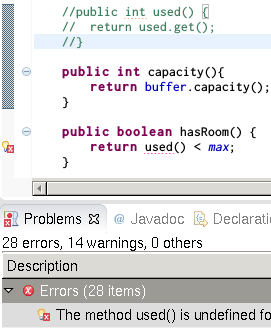
\includegraphics[width=0.22\textwidth]{comment.png}
\caption{The developer comments out a method to trigger errors using the
\textit{lean on the compiler} technique.\label{comment}}
\end{center}
\end{figure}
Navigating to the call sites aims to serve two purposes: to look at the calling
contexts to determine a better name, and to edit each call site to specify
the new method name.

I acknowledge that leaning on the compiler is a common and continuing practice
among software developers. Rather than insisting that developers use an
automated refactoring tool, this paper contributes a new tool
called \pname{}, which aids developers in refactoring
manually by supporting them with navigation assistance.

\section{Background and Related Work}
There are other tools which also help developers refactor manually. Two of them
are
BeneFactor~\cite{bene-factor} and WitchDoctor~\cite{witch-doctor},
which allow developers to start a refactoring manually and then
complete it automatically.
In contrast, \pname{} supports developers in refactoring completely manually.
% TODO: trust is not addressed by these tools.

GhostFactor is a tool which automatically detects
when a developer has completed a manual refactoring, and validates
that the developer has refactored correctly~\cite{ghost-factor}.
In contrast, \pname{} does not help developers with the correctness of
their refactorings, but instead helps them navigate during refactoring.

\section{Approach and Uniqueness}
\pname{} is aimed at supporting the \textit{lean on the compiler} technique
by making it easy for developers to navigate between related errors introduced
during a refactoring. \pname{} achieves this by opening a tab containing
several editors---one for each error (Figure~\ref{mult}).

Consider the example in the introduction, where the developer
wishes to rename a method by first commenting out
the method, so she can find all references to it.
On one of the introduced errors, the developer invokes \pname{} by choosing
the ``Show with other Errors...'' option of Eclipse's Quick Fix
menu (Figure~\ref{quick}).

\begin{figure}[h]
\begin{center}
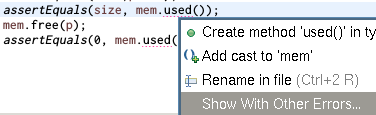
\includegraphics[width=0.35\textwidth]{quick-fix.png}
\caption{Click ``Show with other Errors...'' on an error.\label{quick}}
\end{center}
\end{figure}

Clicking Quick Fix opens \pname{}'s editor (Figure~\ref{mult}). By using the
right-most scrollbar, the developer
can view the twenty errors introduced by this manual refactoring.
The adjacent editors are designed to facilitate two manual refactoring tasks.
First, the developer can view the context of each method reference, to enable
her to choose a more meaningful name. Second, she can use the editors to rename
each call site.

Without \pname{}, the developer had to determine which error messages were
relevant to the refactoring, and then navigate to relevant errors manually. This
process had to be done once for choosing a name, and a second time for making
the change. \pname{} makes this process easier by collecting all errors that
were introduced by the manual refactoring and showing them in a single tab.

\begin{figure}[h]
\begin{center}
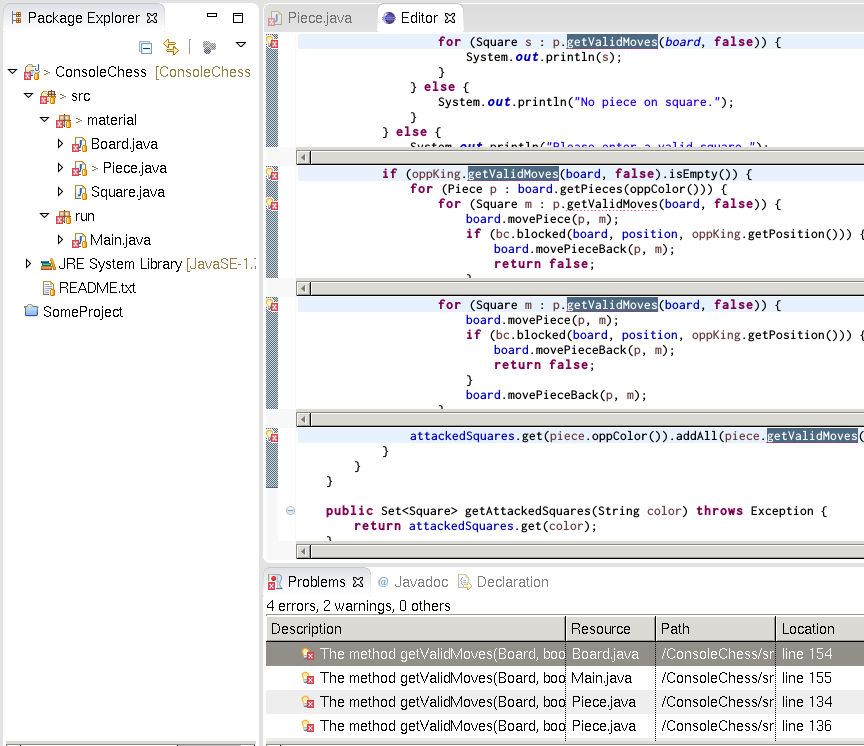
\includegraphics[width=0.45\textwidth]{multiple-editors.png}
\caption{Related errors are each opened in their own editor.\label{mult}}
\end{center}
\end{figure}

\pname{} can be used to accomplish more than a rename refactoring.
\pname{} can assist developers in manually performing the refactorings:
\textit{pull up method}, \textit{push down method}, \textit{add parameter},
\textit{change return type}, and \textit{extract interface}.
In general,
\pname{} helps with tasks where developers must view or edit multiple
references to a particular program element such as a method, variable, or
class.
I implemented \pname{} in Eclipse, and it is freely available on
github at \url{https://github.com/DeveloperLiberationFront/KinEdit}.

\section{Results and Contributions}
I performed a small study to find challenges developers would have with
\pname{}. I asked four participants each to determine a better name for (1) a
method used in across ten files and (2) a private instance variable.  Two
participants used \pname{} to refactor the method, and two used it to refactor
the variable.  When not using the tool, I asked the participants to rename the
identifier with whatever tools they desired, excluding Eclipse's built-in rename
refactoring tool (to simulate as best as possible the demographic who would use
\pname{}) . Both tasks were carried out using the codebase at
\url{https://github.com/raffaeleguidi/DirectMemory}.

The study revealed several interesting insights into how people use \pname{}.
However, due to limited space, I summarize only two of the more interesting
findings in this section.

One result was that the participants were somewhat disoriented when \pname{}
displayed multiple editors for errors located only a few lines apart from each
other. One possible solution is to display all errors which
occur no more than some threshold of lines from each other together in one
editor. Another solution is to display all errors from one file in a single
editor, and use code folding to hide code in between errors.

Another result was a participant who commented that it was difficult to use the
tool to perform a refactoring without a sense of progress. It was not obvious to
him which editors he had visited, edited, and had not looked at yet.  To help
the user, \pname{} might display some sort of progress visuals to indicate which
editors he has placed a cursor in, edited, and never visited.  Color indicators
or a progress meter at the top of \pname{}'s tab may prove to be helpful.

\section{Future Work}
As my study results suggest, significant improvements are necessary to make
\pname{} a robust tool. I plan on improving \pname{} based on my findings, then
performing an experiment to evaluate whether developers can more quickly and
effectively refactor using \pname{}. If accepted, I plan on demonstrating the
revised tool and presenting the results at SPLASH 2015. Along with fixing the
usability issues, I would like to add the following additional capabilities:

\begin{itemize}
  \item Right click an identifier to open all references in \pname{}.
  \item Open \pname{} from Eclipse's find all references and Quick Assist tools.
  \item Always show the declaration of the identifier in the top editor.
  \item Provide hotkeys for users to navigate between editors quickly, and to
      refocus an editor on its primary error.
  \item Allow users to edit all selected references at once.
\end{itemize}

\pname{} enhances the process of manually refactoring. With some additional
work, \pname{} can help developers maintain their code bases while keeping
the developers in complete control.

\appendix
% \section{Appendix Title}
% 
% This is the text of the appendix, if you need one.

\acks
Thank you Dr. Emerson Murphy-Hill for your guidance through writing this
paper during my summer research internship at North Carolina State University.
This material is based upon work supported by the National Science Foundation
under Grant No. 1252995.

% We recommend abbrvnat bibliography style.

\bibliographystyle{abbrvnat}

% The bibliography should be embedded for final submission.

\softraggedright
\bibliography{error-view}

\end{document}
